Der Sprachforscher Stuart M.~Shieber hat aus Beispielen wie dem Satz
\begin{center}
De Jan säit das mer d'Chind em Hans es Hus händ wele laa hälfe aastriiche.
\end{center}
abgeleitet, dass das Schweizderdeutsch grammatische Konstruktionen
zulässt, die auf Wörter der Form
\[
wa^mb^nxc^md^ny
\]
hinaus laufen\footnote{Stuart M.~Shieber,
{\em Evidence against the context-freeness of natural language},
Linguistics and Philosophy, {\bf 8} (1985) 333--343}.
Zeigen Sie, dass diese Sprache nicht kontextfrei ist.

\themaL{Pumping Lemma fur kontextfreie Sprachen}{Pumping Lemma für kontextfreie Sprachen}
\thema{kontextfrei}

\begin{loesung}
\definecolor{darkred}{rgb}{0.8,0,0}
\definecolor{darkgreen}{rgb}{0,0.6,0}
Wir wenden das Pumping Lemma für kontextfreie Sprachen auf die Sprache
\[
L=\{
wa\mathstrut^mb\mathstrut^nxc\mathstrut^md\mathstrut^ny
\;|\; m,n\ge 0
\}
\]
an.
\begin{enumerate}
\item Annahme: $L$ ist kontextfrei.
\item Nach dem Pumping-Lemma gibt es die Pumping-Length $N$.
\item Wir konstruieren das Beispielwort
%\[
%z=wa^Nb^Nxc^Nd^Ny,
%\]
\begin{center}
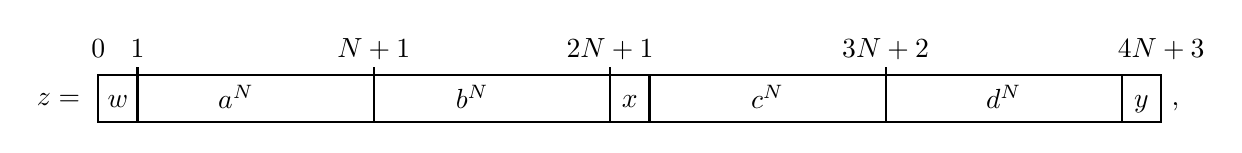
\begin{tikzpicture}[>=latex,thick]
\draw (0,0) rectangle (13.5,0.6);
\draw (0.5,0) -- (0.5,0.7);
\draw (3.5,0) -- (3.5,0.7);
\draw (6.5,0) -- (6.5,0.7);
\draw (7.0,0) -- (7.0,0.6);
\draw (10.0,0) -- (10.0,0.7);
\draw (13.0,0) -- (13.0,0.6);
\node at (0,0.3) [left] {$z=\mathstrut$};
\node at (13.5,0.3) [right] {,\strut};
\node at (0.25,0.28) {$\mathstrut w$};
\node at (1.75,0.28) {$a\mathstrut^N$};
\node at (4.75,0.28) {$b\mathstrut^N$};
\node at (6.75,0.28) {$x\mathstrut$};
\node at (8.5,0.28) {$c\mathstrut^N$};
\node at (11.5,0.28) {$d\mathstrut^N$};
\node at (13.25,0.28) {$y\mathstrut$};

\node at (0,0.6) [above] {$0\mathstrut$};
\node at (0.5,0.6) [above] {$1\mathstrut$};
\node at (3.5,0.6) [above] {$N+1\mathstrut$};
\node at (6.5,0.6) [above] {$2N+1\mathstrut$};
%\node at (7.0,0.6) [above] {$2N+2\mathstrut$};
\node at (10.0,0.6) [above] {$3N+2\mathstrut$};
%\node at (13.0,0.6) [above] {$4N+2\mathstrut$};
\node at (13.5,0.6) [above] {$4N+3\mathstrut$};

\end{tikzpicture}
\end{center}
es ist offensichtlich in der Sprache $L$
und es ist ausreichend lang, dass die Schlussfolgerungen des Pumping-Lemma
darauf anwendbar sind.
\item
Gemäss dem Pumping Lemma gibt es eine Unterteilung
\begin{center}
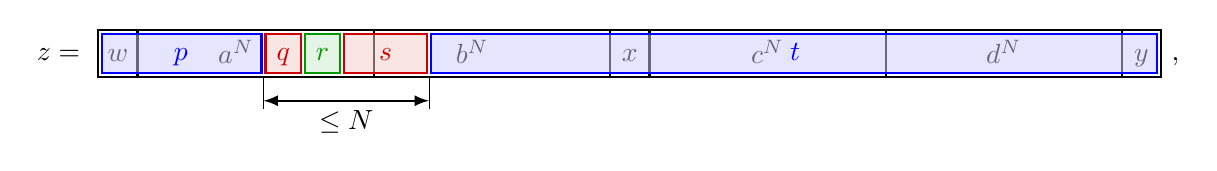
\begin{tikzpicture}[>=latex,thick]
\draw (0,0) rectangle (13.5,0.6);
\draw (0.5,0) -- (0.5,0.6);
\draw (3.5,0) -- (3.5,0.6);
\draw (6.5,0) -- (6.5,0.6);
\draw (7.0,0) -- (7.0,0.6);
\draw (10.0,0) -- (10.0,0.6);
\draw (13.0,0) -- (13.0,0.6);
\node at (0,0.3) [left] {$z=\mathstrut$};
\node at (13.5,0.3) [right] {,\strut};
\node at (0.25,0.28) {$\mathstrut w$};
\node at (1.75,0.28) {$a\mathstrut^N$};
\node at (4.75,0.28) {$b\mathstrut^N$};
\node at (6.75,0.28) {$x\mathstrut$};
\node at (8.5,0.28) {$c\mathstrut^N$};
\node at (11.5,0.28) {$d\mathstrut^N$};
\node at (13.25,0.28) {$y\mathstrut$};
\def\v{2.1}
\def\x{2.6}
\def\y{3.1}
\def\z{4.2}

\fill[color=blue!20,opacity=0.5]
	(0.05,0.05) rectangle ({\v-0.025},0.55);
\draw[color=blue]
	(0.05,0.05) rectangle ({\v-0.025},0.55);
\node[color=blue] at ({0.5*\v},0.3) {$p\mathstrut$};

\fill[color=darkred!20,opacity=0.5]
	({\v+0.025},0.05) rectangle ({\x-0.025},0.55);
\draw[color=darkred]
	({\v+0.025},0.05) rectangle ({\x-0.025},0.55);
\node[color=darkred] at ({0.5*(\v+\x)},0.3) {$q\mathstrut$};

\fill[color=darkgreen!20,opacity=0.5]
	({\x+0.025},0.05) rectangle ({\y-0.025},0.55);
\draw[color=darkgreen]
	({\x+0.025},0.05) rectangle ({\y-0.025},0.55);
\node[color=darkgreen] at ({0.5*(\x+\y)},0.3) {$r\mathstrut$};

\fill[color=darkred!20,opacity=0.5]
	({\y+0.025},0.05) rectangle ({\z-0.025},0.55);
\draw[color=darkred]
	({\y+0.025},0.05) rectangle ({\z-0.025},0.55);
\node[color=darkred] at ({0.5*(\y+\z)},0.3) {$s\mathstrut$};

\fill[color=blue!20,opacity=0.5]
	({\z+0.025},0.05) rectangle (13.45,0.55);
\draw[color=blue]
	({\z+0.025},0.05) rectangle (13.45,0.55);
\node[color=blue] at ({0.5*(\z+13.5)},0.3) {$t\mathstrut$};

\draw[line width=0.3pt] (\v,0) -- (\v,-0.4);
\draw[line width=0.3pt] (\z,0) -- (\z,-0.4);
\draw[<->] (\v,-0.3) -- (\z,-0.3);
\node at ({0.5*(\v+\z)},-0.3) [below] {$\le N$};

\end{tikzpicture}
\end{center}
%\[
%z={\color{blue}p}{\color{darkred}q}{\color{darkgreen}r}{\color{darkred}s}{\color{blue}t},
%\]
wobei $|{\color{darkred}q}{\color{darkgreen}r}{\color{darkred}s}|\le N$
gelten muss.
Es folgt, dass $q$ und $s$ nur jeweils zwei benachbarte der
vier ``langen'' Blöcke $a\mathstrut^N$, $b\mathstrut^N$, $c\mathstrut^N$
oder $d\mathstrut^N$ berühren können.
\item 
Beim Aufpumpen werden zwei benachbarte langen Blöcke verändert.
Die Bedingung, dass alternierende Blöcke, also $a\mathstrut^N$ und
$c\mathstrut^N$ bzw.~$b\mathstrut^N$ und $d\mathstrut^N$ gleich lang
sein müssen, wird nach dem Pumpen daher nicht mehr erfüllt sein.
Ein aufgepumptes Wort wird daher nicht mehr in $L$ sein.
\item Dieser Widerspruch zeigt, dass die Annahme, $L$ sei kontextfrei,
nicht haltbar ist.
\qedhere
\end{enumerate}
\end{loesung}

\begin{diskussion}
Dies bedeutet natürlich nicht, dass Schweizerdeutsch eine nicht
kontextfreie Sprache ist.
In der Wirklichkeit sind die Sätze nämlich immer von beschränkter Länge,
die Exponenten $n$ und $m$ können daher nicht beliebig gross sein.
Das müssen Sie aber, denn der Pumping-Lemma-Beweis verlangt, dass man
$n=m=N$ setze können muss, wobei die Pumping-Length $N$ eben sehr gross
sein kann.
\end{diskussion}

\begin{bewertung}
Jeder Punkt des Pumping-Lemma-Beweises ein Punkt:
Annahme ({\bf A}), Pumping Length ({\bf N}), Beispielwort ({\bf W}),
Zerlegung ({\bf Z}), Widerspruch beim Pumpen ({\bf P}), 
Folgerung ({\bf F}).
Der Punkt ({\bf Z}) wird nur gegeben, wenn zum Beispiel aus dem nachfolgenden
Pumpschritt klar wird, dass es mehrere mögliche Unterteilungen gibt.
\end{bewertung}

